\documentclass[12pt,a4paper]{article}

\usepackage[utf8]{inputenc}
\usepackage[T1]{fontenc}
\usepackage[brazil]{babel}
\usepackage{lmodern}
\usepackage[margin=2.5cm]{geometry}
\usepackage{graphicx}
\usepackage{booktabs}
\usepackage{amsmath}
\usepackage{float}
\usepackage{listings}
\usepackage{xcolor}
\usepackage[hidelinks]{hyperref}
\usepackage{setspace}
\newcommand{\SI}[2]{\mbox{#1\,#2}}
\onehalfspacing

\lstset{
  basicstyle=\ttfamily\small,
  breaklines=true,
  frame=single,
  backgroundcolor=\color{gray!8},
  columns=fullflexible
}

\title{\textbf{Avaliação da Capacidade Máxima de Transmissão de uma\\
Aplicação de Chat TCP Multithread: Clientes $\rightarrow$ Servidor}}
\author{Felipe Baz Mitsuishi\\
RA 140867\\
Universidade Federal de São Paulo (UNIFESP)\\
\texttt{felipe.mitsuishi@unifesp.br}}
\date{3 de novembro de 2026}

\begin{document}
\maketitle

\begin{abstract}
Este trabalho avalia a taxa de transmissão agregada máxima que um servidor de
chat TCP, implementado em C com um modelo de uma thread por conexão, é capaz de
receber de um número variável de clientes simultâneos (1 a 10). A aplicação
original foi modificada para incluir um modo de benchmark, no qual os clientes
transmitem blocos de dados continuamente por um intervalo definido, sem
interação manual, e o servidor contabiliza os bytes efetivamente recebidos em
cada thread, por meio de contadores independentes, dentro de uma janela de
medição fixa. Cada configuração foi repetida cinco vezes com blocos de
\SI{64}{KiB}. Observou-se escalabilidade quase linear até dois clientes
($\approx$\,\SI{47}{Gbps}), saturação a partir de quatro clientes, com
patamar entre 76 e \SI{85}{Gbps} (pico médio de \SI{84{,}75}{Gbps} com seis
clientes), e forte influência do tamanho do bloco: \SI{25{,}8}{Gbps} com
blocos de \SI{512}{B} contra \SI{90{,}0}{Gbps} com \SI{4}{KiB}, para dez
clientes. Como cliente e servidor compartilham a mesma máquina e a interface de
\textit{loopback}, os resultados caracterizam o limite do processamento da
pilha TCP e do \textit{software}, e não de um enlace físico.
\end{abstract}

\section{Introdução}

Servidores de rede baseados em sockets TCP e em uma thread por conexão são um
padrão didático e prático para aplicações de comunicação. Entretanto, a
capacidade agregada de recepção de tais servidores depende da interação entre
o número de conexões, o custo de chamadas de sistema, a política de
escalonamento do sistema operacional e a pilha TCP. O objetivo deste trabalho é
quantificar empiricamente essa capacidade, variando o número de clientes
simultâneos de 1 a 10, e identificar os limites e gargalos observados.

\section{Implementação}

O código-base é um chat TCP em C (POSIX \textit{sockets} e \textit{pthreads}),
no qual o servidor cria uma thread por cliente aceito. Foram realizadas as
modificações a seguir, preservando o comportamento original quando os
argumentos de benchmark não são fornecidos.

\paragraph{Servidor.} Ao ser iniciado com \texttt{--bench N}, o servidor aguarda
$N$ clientes que se identificam com a linha \texttt{/bench <nome>}. Uma
\textit{barreira} (\texttt{pthread\_mutex} e \texttt{pthread\_cond}) sincroniza o
início: quando o $N$-ésimo cliente chega, todos recebem
\texttt{GO <duração>} e uma thread medidora é disparada. Cada thread de
atendimento lê o socket com um \textit{buffer} de \SI{256}{KiB} e acumula o
número de bytes lidos em um contador atômico próprio, alinhado a linhas de
\SI{64}{B} para evitar \textit{false sharing}. Assim, não há \textit{lock} no
caminho crítico de recepção.

\paragraph{Cliente.} O cliente, com \texttt{--bench <nome> [bloco]}, aguarda o
\texttt{GO} e transmite blocos de tamanho fixo (preenchidos com dados
constantes) em laço contínuo, com \texttt{send} completo (\texttt{send\_all}),
até expirar a duração informada pelo servidor. Em seguida, executa
\texttt{shutdown(SHUT\_WR)}.

\paragraph{Automação.} O \textit{script} \texttt{scripts/run\_experiments.sh} executa,
para cada $N$ e cada repetição, um servidor novo e $N$ clientes simultâneos,
registrando o resultado em CSV. O \textit{script} \texttt{scripts/analyze.py} produz as
tabelas e os gráficos deste relatório.

\section{Ambiente Experimental}

\begin{table}[H]
\centering
\caption{Características da máquina e do ambiente de execução.}
\label{tab:ambiente}
\begin{tabular}{ll}
\toprule
\textbf{Item} & \textbf{Especificação}\\
\midrule
Processador & AMD Ryzen 5 5600X (6 núcleos, 12 threads lógicas)\\
Memória RAM (hospedeiro) & \SI{32}{GB}\\
Memória visível ao WSL2 & \SI{15{,}6}{GiB} (12 vCPUs)\\
SO hospedeiro & Windows 11 Home 10.0.26200\\
SO de execução & Ubuntu 24.04 (WSL2, \textit{kernel} Linux 6.6.87.2-microsoft-standard-WSL2)\\
Compilador & GCC 13.3.0 (Ubuntu 13.3.0-6ubuntu2$\sim$24.04.1)\\
Opções de compilação & \texttt{-O2 -Wall -Wextra -pthread}\\
Máquinas & 1 (cliente e servidor no mesmo hospedeiro)\\
Rede & Interface de \textit{loopback} (127.0.0.1), TCP/IPv4\\
\textit{Buffers} TCP (\texttt{tcp\_rmem}) & 4096 / 131072 / 6291456 B (mín/padrão/máx)\\
\textit{Buffers} TCP (\texttt{tcp\_wmem}) & 4096 / 16384 / 4194304 B (mín/padrão/máx)\\
\bottomrule
\end{tabular}
\end{table}

Toda a comunicação ocorreu pela interface de \textit{loopback} dentro de uma
única máquina virtual (WSL2). Não há, portanto, enlace físico, \textit{switch}
ou placa de rede envolvidos, e as taxas medidas refletem o custo
computacional do \textit{software} e da pilha TCP do \textit{kernel}.

\section{Metodologia}

\subsection{Parâmetros dos experimentos}

\begin{table}[H]
\centering
\caption{Parâmetros experimentais.}
\label{tab:params}
\begin{tabular}{ll}
\toprule
\textbf{Parâmetro} & \textbf{Valor}\\
\midrule
Clientes simultâneos ($N$) & 1, 2, \ldots, 10\\
Tamanho do bloco (experimento principal) & \SI{65536}{B} (\SI{64}{KiB})\\
Aquecimento (descartado) & \SI{2}{s}\\
Janela de medição & \SI{10}{s}\\
Folga final de transmissão & \SI{1}{s}\\
Duração de envio por cliente & \SI{13}{s}\\
Repetições (experimento principal) & 5 por valor de $N$ (50 execuções)\\
Varredura de blocos ($N=10$) & \SI{512}{B}, \SI{4}{KiB}, \SI{16}{KiB}, \SI{64}{KiB}, \SI{256}{KiB}\\
Repetições (varredura de blocos) & 3 (5 para \SI{64}{KiB})\\
\bottomrule
\end{tabular}
\end{table}

\subsection{Procedimentos para comparabilidade}

Para garantir que as configurações sejam comparáveis entre si, adotaram-se os
seguintes procedimentos:

\begin{itemize}
  \item \textbf{Início sincronizado:} a barreira do servidor libera todos os
  clientes simultaneamente, de modo que todos transmitam ao mesmo tempo.
  \item \textbf{Aquecimento descartado:} os primeiros \SI{2}{s} (abertura de
  conexões, crescimento das janelas TCP, \textit{page faults}) não entram na
  medição.
  \item \textbf{Janela de medição interna:} apenas o intervalo
  $[t_0,t_1]$ de \SI{10}{s} é considerado; os clientes continuam transmitindo
  por mais \SI{1}{s}, de modo que o encerramento de conexões não interfere.
  \item \textbf{Processo novo por execução:} um servidor é iniciado a cada
  repetição, eliminando estado residual.
  \item \textbf{Mesmo binário e mesmos parâmetros:} somente $N$ (ou o tamanho do
  bloco, na varredura específica) varia entre configurações.
  \item \textbf{Relógio monotônico:} os tempos usam
  \texttt{CLOCK\_MONOTONIC}, imune a ajustes do relógio do sistema.
  \item \textbf{Validação cruzada:} a soma das taxas reportadas pelos clientes
  coincide com a medida pelo servidor (por exemplo, em um teste preliminar
  com dois clientes: $\approx$\,\SI{50{,}2}{Gbps} no servidor contra
  25,17 + 25,05 no cliente).
  \item \textbf{Descarte de execução inválida:} uma primeira rodada foi
  descartada integralmente porque duas instâncias do \textit{script}
  executaram simultaneamente e disputaram a mesma porta. Todos os resultados
  apresentados provêm de uma rodada com uma única instância ativa.
\end{itemize}

\subsection{Cálculo da taxa de transmissão agregada}

Seja $c_i(t)$ o contador de bytes recebidos pela thread que atende o cliente
$i$ até o instante $t$, incrementado a cada retorno bem-sucedido de
\texttt{recv} pelo número de bytes efetivamente lidos (e não pelo que o cliente
declara ter enviado). Cada contador é atômico e exclusivo de sua thread. A
thread medidora lê o total
\begin{equation}
B(t)=\sum_{i=1}^{N} c_i(t)
\end{equation}
no instante $t_0$ (após o aquecimento) e no instante $t_1$ (após a janela de
medição). A taxa agregada é
\begin{equation}
R=\frac{\bigl(B(t_1)-B(t_0)\bigr)\cdot 8}{(t_1-t_0)\cdot 10^{6}}\quad[\text{Mbps}],
\end{equation}
em que $t_1-t_0$ é medido com \texttt{clock\_gettime}
(\texttt{CLOCK\_MONOTONIC}) e é de aproximadamente \SI{10}{s}. Adota-se
$1\,\text{Mbps}=10^{6}$ bits/s. As leituras são feitas com ordenação de
memória relaxada, o que é suficiente, pois os contadores são monotônicos e a
diferença $B(t_1)-B(t_0)$ é tolerante a pequenas defasagens entre as leituras
individuais (erro de, no máximo, alguns blocos por thread, desprezível frente
a $\sim\!10^{11}$ bytes por janela). O valor reportado por $N$ é a média das
repetições, acompanhada do desvio-padrão amostral, do mínimo e do máximo.

\section{Resultados}

\subsection{Throughput agregado versus número de clientes}

\begin{table}[H]
\centering
\caption{Throughput agregado recebido pelo servidor (bloco de \SI{64}{KiB},
5 repetições por $N$). Valores em Mbps; a última coluna é a média por cliente
em Gbps.}
\label{tab:main}
\begin{tabular}{rrrrrr}
\toprule
$N$ & Média (Mbps) & Desvio & Mín & \textbf{Máx (Mbps)} & Por cliente (Gbps)\\
\midrule
1  & 24\,105 & 153   & 23\,949 & 24\,295 & 24,11\\
2  & 47\,139 & 289   & 46\,859 & 47\,534 & 23,57\\
3  & 65\,854 & 1\,256 & 64\,385 & 67\,297 & 21,95\\
4  & 77\,683 & 823   & 76\,811 & 79\,018 & 19,42\\
5  & 79\,938 & 3\,370 & 75\,812 & 82\,646 & 15,99\\
6  & 84\,750 & 827   & 84\,043 & 86\,087 & 14,13\\
7  & 78\,058 & 4\,124 & 72\,283 & 82\,184 & 11,15\\
8  & 82\,382 & 1\,036 & 81\,206 & 83\,993 & 10,30\\
9  & 76\,298 & 1\,147 & 75\,156 & 77\,901 & 8,48\\
10 & 80\,141 & 1\,731 & 77\,315 & 81\,560 & 8,01\\
\bottomrule
\end{tabular}
\end{table}

\subsection{Throughput agregado máximo versus número de clientes}

\begin{table}[H]
\centering
\caption{Número de clientes simultâneos (1 a 10) versus throughput agregado
máximo observado entre as 5 repetições (bloco de \SI{64}{KiB}), em Mbps.
Inclui-se a média para referência.}
\label{tab:max}
\begin{tabular}{rrr}
\toprule
Clientes & \textbf{Throughput máximo (Mbps)} & Média (Mbps)\\
\midrule
1  & 24\,295 & 24\,105\\
2  & 47\,534 & 47\,139\\
3  & 67\,297 & 65\,854\\
4  & 79\,018 & 77\,683\\
5  & 82\,646 & 79\,938\\
6  & 86\,087 & 84\,750\\
7  & 82\,184 & 78\,058\\
8  & 83\,993 & 82\,382\\
9  & 77\,901 & 76\,298\\
10 & 81\,560 & 80\,141\\
\bottomrule
\end{tabular}
\end{table}

\begin{figure}[H]
\centering
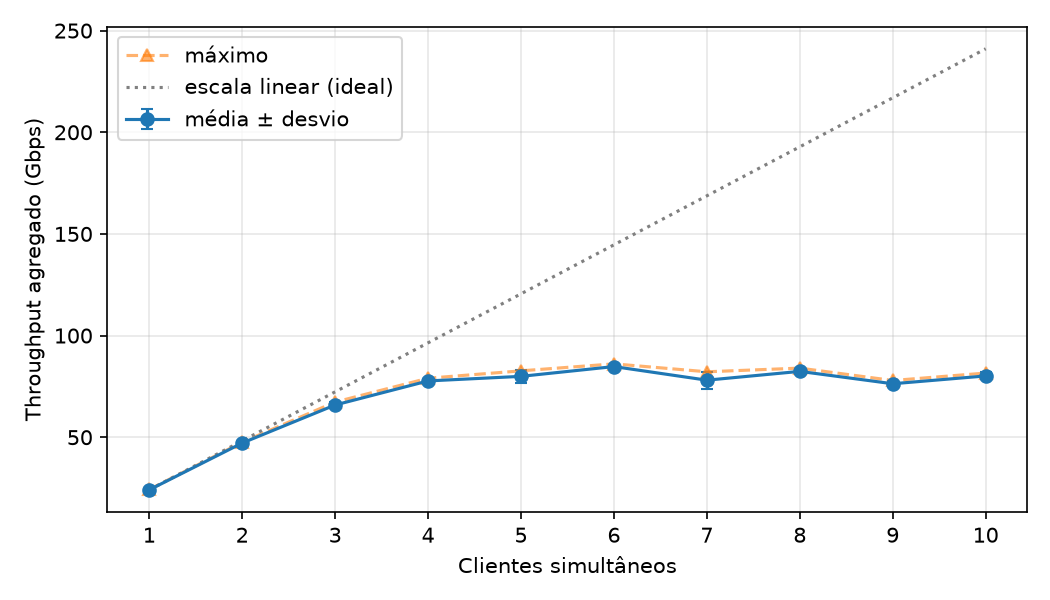
\includegraphics[width=0.85\textwidth]{../figures/throughput.png}
\caption{Throughput agregado (média $\pm$ desvio-padrão e máximo) em função do
número de clientes simultâneos. A linha pontilhada representa a escala linear
ideal a partir do valor com um cliente.}
\label{fig:thr}
\end{figure}

\begin{figure}[H]
\centering
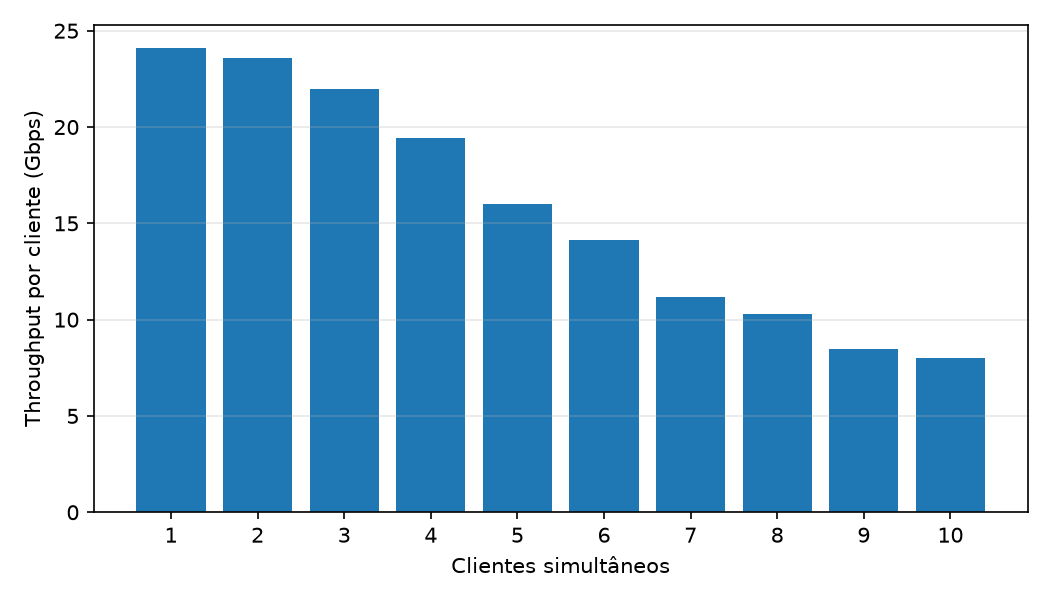
\includegraphics[width=0.85\textwidth]{../figures/per_client.png}
\caption{Throughput médio por cliente em função do número de clientes.}
\label{fig:perclient}
\end{figure}

\subsection{Influência do tamanho do bloco ($N=10$)}

\begin{table}[H]
\centering
\caption{Throughput agregado com 10 clientes para diferentes tamanhos de bloco.}
\label{tab:blocks}
\begin{tabular}{rrrrr}
\toprule
Bloco (B) & Reps. & Média (Mbps) & Desvio & Máx (Mbps)\\
\midrule
512     & 3 & 25\,796 & 2\,108 & 27\,088\\
4\,096  & 3 & 90\,001 & 4\,899 & 95\,615\\
16\,384 & 3 & 84\,406 & 652    & 85\,121\\
65\,536 & 5 & 80\,141 & 1\,731 & 81\,560\\
262\,144 & 3 & 73\,325 & 5\,699 & 79\,822\\
\bottomrule
\end{tabular}
\end{table}

\begin{figure}[H]
\centering
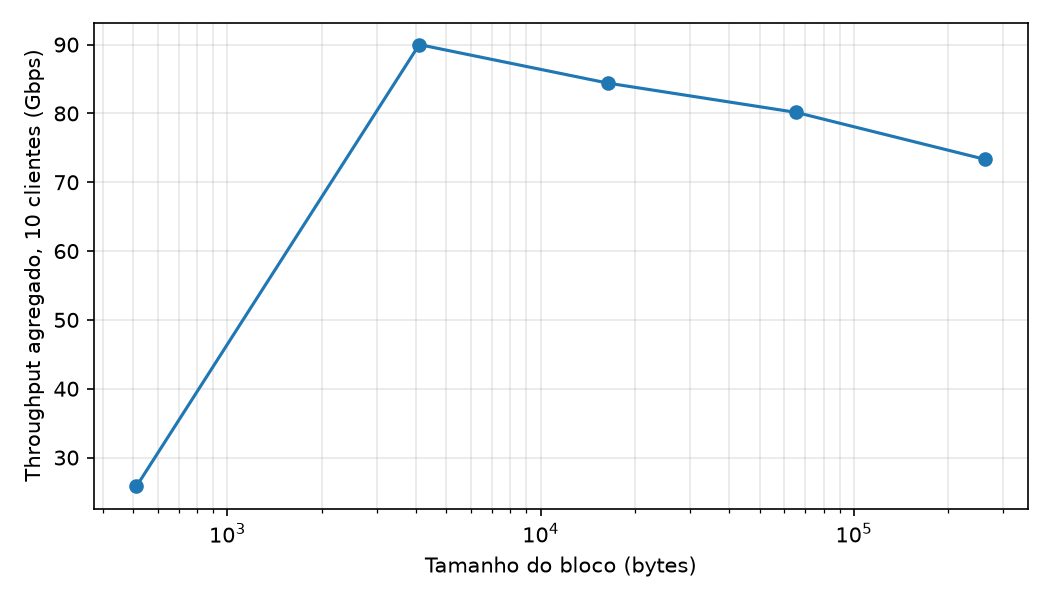
\includegraphics[width=0.85\textwidth]{../figures/blocks.png}
\caption{Throughput agregado com 10 clientes em função do tamanho do bloco
(eixo horizontal logarítmico).}
\label{fig:blocks}
\end{figure}

\section{Discussão}

\paragraph{Impacto do número de clientes.} Com um único cliente, o servidor
recebeu em média \SI{24{,}1}{Gbps}. O ganho foi quase linear até dois clientes
($1{,}96\times$), mas com três ($2{,}73\times$) e quatro clientes
($3{,}22\times$) a eficiência de escala caiu para 91\% e 80\%,
respectivamente. A partir de quatro clientes, o throughput agregado deixa de
crescer de forma significativa e oscila entre 76 e \SI{85}{Gbps}, com
pico médio em seis clientes (\SI{84{,}75}{Gbps}, $3{,}52\times$ o valor com um
cliente). Entre quatro e dez clientes, a variação observada é pequena em
relação à ampliação de 2,5 vezes na carga oferecida, e a taxa por cliente cai
de 19,4 para \SI{8{,}0}{Gbps} (Figura~\ref{fig:perclient}). Portanto,
adicionar clientes além de quatro não aumenta a capacidade do servidor; apenas
redistribui uma capacidade já saturada.

\paragraph{Variabilidade.} Os desvios-padrão são pequenos para $N\le 2$
(inferiores a 1\%) e maiores em alguns pontos de saturação ($N=5$: 4,2\%;
$N=7$: 5,3\%). A não monotonicidade na região de platô (por exemplo, $N=7$ e
$N=9$ abaixo de $N=6$ e $N=8$) está dentro da dispersão entre repetições e,
com apenas cinco amostras, não permite afirmar uma tendência real entre esses
valores. Em saturação, a distribuição das threads entre os núcleos pelo
escalonador torna-se fator de ruído.

\paragraph{Impacto do tamanho do bloco.} Com blocos de \SI{512}{B}, o
throughput caiu para \SI{25{,}8}{Gbps}, cerca de $3{,}5$ vezes menos que o
obtido com \SI{4}{KiB}. Com blocos pequenos, o número de chamadas
\texttt{send}/\texttt{recv} por byte transferido aumenta, e o custo fixo por
chamada (transição \textit{user}/\textit{kernel}, processamento do segmento TCP)
passa a dominar. O melhor resultado ocorreu com \SI{4}{KiB}
(\SI{90{,}0}{Gbps}, máximo de \SI{95{,}6}{Gbps}); acima disso, o throughput decresce
de forma gradual (84,4, 80,1 e \SI{73{,}3}{Gbps} para 16, 64 e
\SI{256}{KiB}). Uma hipótese compatível com esse comportamento, que não foi
verificada isoladamente, é que blocos muito grandes
excedam a capacidade das caches de dados dos núcleos e dos \textit{buffers} de
socket, aumentando o tráfego de memória. Assim, o resultado do experimento
principal (\SI{64}{KiB}) não representa o máximo absoluto do servidor:
\SI{4}{KiB} entregou cerca de 12\% a mais com dez clientes.

\subsection{Perfilamento com \texttt{perf}}

Para verificar empiricamente os gargalos, os cenários principais foram
reexecutados sob o \texttt{perf} (versão 6.8, contadores de hardware
disponíveis no \textit{guest}), com amostragem do sistema inteiro
(\texttt{-a}, \SI{999}{Hz}, com pilha de chamadas) durante a janela de medição.
As estatísticas globais (\texttt{perf stat}) cobrem \SI{4}{s} da janela
(de 3 a \SI{7}{s}); a amostragem de símbolos cobre os \SI{3}{s} seguintes. O uso
de CPU por categoria foi obtido de \texttt{/proc/stat} na mesma janela de
\SI{4}{s}. Cada cenário foi perfilado uma única vez; a instrumentação
perturba a execução (as taxas medidas sob \texttt{perf} diferiram de $-11\%$ a
$+13\%$ das médias da Tabela~\ref{tab:main}), de modo que os percentuais são
indicativos e não possuem intervalo de confiança.

\begin{table}[H]
\centering
\caption{Uso de CPU e contadores globais sob \texttt{perf} (12 CPUs lógicas;
bloco de \SI{64}{KiB}, exceto onde indicado). \textit{User}, \textit{sys},
\textit{softirq} e \textit{idle} em \% do tempo total de CPU; IPC =
instruções por ciclo; troca de contexto (CS) em milhares por segundo.}
\label{tab:perf}
\small
\begin{tabular}{lrrrrrrrr}
\toprule
Cenário & Gbps & user & sys & softirq & idle & IPC & CS (mil/s) \\
\midrule
$N=1$            & 24,7 & 0,0 & 10,1 & 1,6 & 88,3 & 0,24 & 4,9\\
$N=4$            & 72,9 & 0,3 & 43,6 & 4,4 & 51,7 & 0,18 & 11,0\\
$N=6$            & 75,5 & 0,5 & 69,6 & 6,5 & 23,3 & 0,12 & 9,3\\
$N=10$           & 76,6 & 0,7 & 90,9 & 6,9 & 1,5  & 0,10 & 6,2\\
$N=10$, 512\,B   & 29,2 & 9,5 & 70,4 & 5,5 & 14,5 & 0,52 & 100,1\\
$N=10$, 4\,KiB   & 96,4 & 5,1 & 83,3 & 9,7 & 1,9  & 0,35 & 155,6\\
$N=10$, 256\,KiB & 74,8 & 0,5 & 87,9 & 9,1 & 2,5  & 0,10 & 6,7\\
\bottomrule
\end{tabular}
\end{table}

\begin{table}[H]
\centering
\caption{Distribuição das amostras do \texttt{perf record} (\% das amostras do
sistema): participação por processo e principais funções do \textit{kernel}.
\texttt{copyout} (servidor) é a cópia \textit{kernel}$\to$usuário feita em
\texttt{recv}; \texttt{copyin} (cliente), a cópia usuário$\to$\textit{kernel}
feita em \texttt{send}; \texttt{clear\_page\_erms} (cliente), a
zeragem de páginas.}
\label{tab:perfsym}
\small
\begin{tabular}{lrrrrr}
\toprule
Cenário & Servidor & Cliente & \texttt{copyout} & \texttt{copyin} & \texttt{clear\_page\_erms}\\
\midrule
$N=1$            & 72,1 & 25,6 & 57,6 & 4,6 & 3,4\\
$N=4$            & 67,0 & 29,1 & 55,6 & 3,4 & 10,3\\
$N=6$            & 64,2 & 33,1 & 54,3 & 3,1 & 14,5\\
$N=10$           & 66,0 & 32,8 & 54,1 & 3,4 & 15,7\\
$N=10$, 512\,B   & 5,0  & 92,1 & $<0{,}3$ & 3,7 & $<0{,}3$\\
$N=10$, 4\,KiB   & 35,9 & 62,2 & 27,5 & 3,0 & 4,0\\
$N=10$, 256\,KiB & 65,7 & 33,0 & 53,2 & 5,0 & 15,3\\
\bottomrule
\end{tabular}
\end{table}

\paragraph{Principais constatações.}
\begin{enumerate}
  \item \textbf{O tempo está no \textit{kernel}, não na aplicação.} O tempo
  em modo usuário é inferior a 1\% para blocos $\ge$\,\SI{64}{KiB}; mais de
  90\% do tempo de CPU com $N=10$ é \textit{sys} e cerca de 7\% é \textit{softirq}.
  Código do servidor (laço de \texttt{recv} e contador atômico) não é
  limitante.
  \item \textbf{A cópia de dados domina.} Em todos os cenários com blocos
  $\ge$\,\SI{64}{KiB}, entre 53\% e 58\% das amostras de todo o sistema estão em
  \texttt{copyout}, ou seja, na cópia \textit{kernel}$\to$usuário executada
  pelo servidor. O IPC cai de 0,24 ($N=1$) para 0,10 ($N=10$), padrão típico de
  código limitado por acessos à memória (ciclos parados esperando dados).
  \item \textbf{O patamar não é saturação simples de CPU.} Com $N=4$, 51,7\%
  das CPUs lógicas estavam ociosas e, com $N=6$, 23,3\%, mas o throughput já
  estava em 73 a \SI{76}{Gbps}. A eficiência por CPU ocupada
  (throughput dividido pelo número de CPUs lógicas ocupadas, obtido de
  $12\times(1-\text{idle})$) cai de \SI{17,6}{Gbps/CPU} ($N=1$) para
  12,6 ($N=4$), 8,2 ($N=6$) e \SI{6,5}{Gbps/CPU} ($N=10$). Ou seja, CPUs
  adicionais são consumidas sem produzir banda proporcional, o que é compatível
  com disputa por recurso compartilhado --- largura de banda de memória, caches
  e execução das duas threads lógicas de um mesmo núcleo físico (SMT; há 6
  núcleos físicos). Estes dados não permitem separar qual desses recursos é o
  fator preponderante; isso exigiria, por exemplo, contadores de
  tráfego de memória ou testes com SMT desabilitado.
  \item \textbf{Zeragem de páginas no lado transmissor.}
  \texttt{clear\_page\_erms} no cliente cresce de 3,4\% ($N=1$) para 15,7\%
  ($N=10$) das amostras, sugerindo pressão de alocação de memória
  (\textit{buffers} de envio) com muitos fluxos. Não foi investigada a causa
  exata.
  \item \textbf{Blocos pequenos: custo por chamada de sistema.} Com
  \SI{512}{B}, \texttt{copyout} e \texttt{clear\_page\_erms} desaparecem do topo;
  o lado cliente concentra 92,1\% das amostras, dominadas por
  \texttt{tcp\_sendmsg\_locked}, \texttt{\_\_sys\_sendto}, \texttt{\_\_local\_bh\_enable\_ip}
  e \texttt{tcp\_write\_xmit}, o tempo em modo usuário sobe para 9,5\% e as
  trocas de contexto, para cerca de 100 mil/s (contra
  6 mil/s com \SI{64}{KiB}). O gargalo desloca-se para o
  processamento por chamada/segmento no \textit{sender}, e o servidor fica
  com somente 5,0\% das amostras.
  \item \textbf{Ponto ótimo em \SI{4}{KiB}.} Com esse bloco, \texttt{copyout}
  cai para 27,5\% das amostras e a taxa chega a \SI{96,4}{Gbps} sob
  \texttt{perf}. Uma explicação plausível, não testada isoladamente, é que
  blocos que cabem nas caches de dados dos núcleos reduzem as
  falhas de cache e o tráfego de memória, ao custo de mais chamadas.
  \item \textbf{Escalonamento e migração não limitam.} Para blocos de
  \SI{64}{KiB}, as trocas de contexto ficam entre 5 e 11 mil/s e as
  migrações de CPU, abaixo de 0,5 mil/s (1254 em \SI{4}{s} com $N=10$); o
  modelo de uma thread por conexão não é o limitante para $N\le 10$.
\end{enumerate}

\section{Limites Observados e Possíveis Gargalos}

\paragraph{Limite observado.} Nos experimentos principais, o limite superior de
throughput agregado foi de \SI{84{,}75}{Gbps} (média, $N=6$) e de
\SI{86{,}09}{Gbps} (máximo individual, $N=6$). Na varredura de blocos, o
limite foi \SI{90{,}0}{Gbps} (média) e \SI{95{,}6}{Gbps} (máximo individual)
com blocos de \SI{4}{KiB} e $N=10$. Todos esses valores são muito superiores à
capacidade de enlaces Ethernet comuns (1 a \SI{10}{Gbps}); em uma rede real,
o gargalo seria a camada física, e não o \textit{software}.

\paragraph{Gargalos identificados.} A partir do perfilamento (Seção anterior),
classificam-se os fatores inicialmente hipotetizados como:
\begin{enumerate}
  \item \textbf{Confirmado --- cópias de memória no \textit{kernel}.} Cerca de
  54\% das amostras do sistema estão em \texttt{copyout} com blocos grandes, com
  IPC de 0,10. É o principal consumidor de CPU e o fator que limita a vazão
  por byte.
  \item \textbf{Parcialmente confirmado --- recursos compartilhados
  (memória/caches/SMT) em vez de CPU pura.} O platô ocorre com CPUs ainda ociosas
  ($N=4$ e $N=6$), e a eficiência por CPU ocupada cai $\approx$\,2,7 vezes entre
  $N=1$ e $N=10$. A identificação de qual recurso específico limita requer
  medições adicionais. Com $N=10$, a CPU chega a 98,5\% de uso
  (clientes e servidor compartilham a mesma máquina), de modo que o patamar
  mede conjuntamente transmissão e recepção.
  \item \textbf{Confirmado --- custo por chamada de sistema com blocos pequenos
  (\SI{512}{B}):} 92\% das amostras no lado transmissor, 100 mil trocas de
  contexto/s.
  \item \textbf{Não confirmado/inconclusivo --- virtualização.} O tempo de
  \textit{steal} observado no \textit{guest} foi 0\%, mas isso não exclui custo
  da camada Hyper-V (por exemplo, no escalonamento dos núcleos virtuais), que
  não é visível por esse indicador.
  \item \textbf{Descartado como limitante ($N\le 10$) --- modelo de uma thread por
  conexão:} trocas de contexto e migrações baixas, e tempo em modo usuário
  inferior a 1\%. O comportamento com centenas de conexões não foi testado.
\end{enumerate}

\section{Ameaças à Validade}

\begin{itemize}
  \item \textbf{Ambiente único e sem rede física:} os resultados não se
  generalizam para clientes remotos nem para \textit{hardware} de rede.
  \item \textbf{Concorrência com o sistema hospedeiro:} o Windows e outros
  processos podem ter consumido CPU durante os testes; não houve isolamento
  de núcleos nem fixação de afinidade (\textit{CPU pinning}).
  \item \textbf{Número limitado de repetições:} cinco repetições (três na
  varredura de blocos) fornecem estimativas de média e desvio com baixa
  potência estatística; não foram calculados intervalos de confiança.
  \item \textbf{Carga sintética:} os dados são constantes e unidirecionais; o
  tráfego real de chat (mensagens curtas, \textit{broadcast}) seria muito
  distinto.
  \item \textbf{Cliente e servidor competem por recursos,} subestimando a
  capacidade do servidor isolado.
\end{itemize}

\section{Conclusão}

O servidor de chat TCP multithread modificado alcançou, em \textit{loopback},
\SI{24{,}1}{Gbps} com um cliente e saturou a partir de quatro clientes, com
patamar de 76 a \SI{85}{Gbps} (pico médio de \SI{84{,}75}{Gbps} com seis
clientes, bloco de \SI{64}{KiB}). Acrescentar clientes acima desse ponto reduz
a taxa individual sem elevar a taxa agregada. O tamanho do bloco mostrou-se
determinante: \SI{4}{KiB} entregou \SI{90{,}0}{Gbps} com dez clientes, contra
\SI{25{,}8}{Gbps} para \SI{512}{B}. Como trabalho futuro, recomenda-se repetir
o experimento com cliente e servidor em máquinas distintas, com afinidade de
CPU, mais repetições, SMT desabilitado e contadores de tráfego de memória
para separar o efeito de cada recurso compartilhado. O perfilamento com
\texttt{perf} indicou que a cópia \textit{kernel}$\to$usuário
(\texttt{copyout}, $\approx$\,54\% das amostras) domina o custo com blocos
grandes e que o platô ocorre com CPUs ainda ociosas, isto é, por disputa de
recursos compartilhados, e não por saturação simples de CPU.

\section*{Código-fonte e Instruções}

\noindent Servidor e cliente modificados (repositório único):\\
\url{https://github.com/Felipe-Baz/tcp-chat-throughput-unifesp}\\
Servidor: \texttt{src/chat\_server.c}; cliente: \texttt{src/chat\_client.c}.

\medskip
\noindent\textbf{Compilação} (Linux/WSL2):
\begin{lstlisting}
sh scripts/build.sh      # gera bin/chat_server e bin/chat_client
\end{lstlisting}

\noindent\textbf{Execução manual} ($N=10$, \SI{2}{s} de aquecimento, \SI{10}{s} de medição):
\begin{lstlisting}
bin/chat_server 5000 --bench 10 2 10
bin/chat_client 127.0.0.1 5000 --bench c1 65536     # um por cliente
\end{lstlisting}

\noindent\textbf{Experimento completo e análise:}
\begin{lstlisting}
REPS=5 sh scripts/run_experiments.sh results.csv
python3 scripts/analyze.py
\end{lstlisting}

\noindent Sem o argumento \texttt{--bench}, servidor e cliente funcionam como o
chat original (\texttt{./chat\_server 5000}; \texttt{./chat\_client 127.0.0.1 5000}).

\end{document}
